\subsection{Застосування алгоритму Б-К для отримання маски рухомих об'єктів}

Введемо поняття \textbf{маски рухомих об'єктів}.

Маскою рухомих об'єктів кадру \(F^{i}\) будемо називати бінарне
зображення \(B^{i}:P \rightarrow \left\{ 0,1 \right\}\), де тим
пікселям, в яких на відповідному кадрі \(F^{i}\) було помічено рух,
відповідає одиниця, а іншим відповідає нуль. Для обраного користувачем
кроку \(s > 0\) на двох кадрах \(F^{i}\) і \(F^{i + s}\) рухомі об'єкти
являють собою підмножину пікселів, колір яких було змінено більше, ніж
на певне значення, з урахуванням зміни кольорів у сусідніх пікселях.
Тобто, якщо рухомий об'єкт складається з одного пікселя, його рух може
бути проігнорованим в залежності від обраних користувачем налаштувань,
про які йдеться мова далі; аналогічно, якщо рухомий об'єкт на кадрі
містить нерухомі «дірки» (пікселі, де колір не змінився), вони можуть
вважатися частиною рухомого об'єкту.

\begin{figure}[H]
    \centering
    \begin{subfigure}[b]{0.55\textwidth}
      \centering
      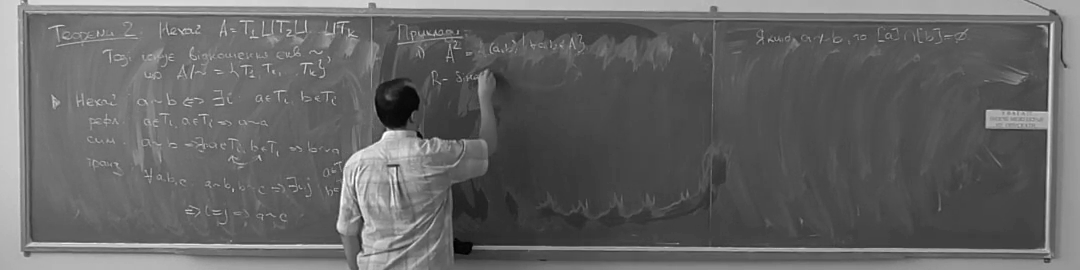
\includegraphics[width=\textwidth]{images/prev_yakovlev}
      \caption{Попередній кадр
      \label{fig:yakovlev:bk_examples:a}
      }
    \end{subfigure}

    \begin{subfigure}[b]{0.55\textwidth}
        \centering
        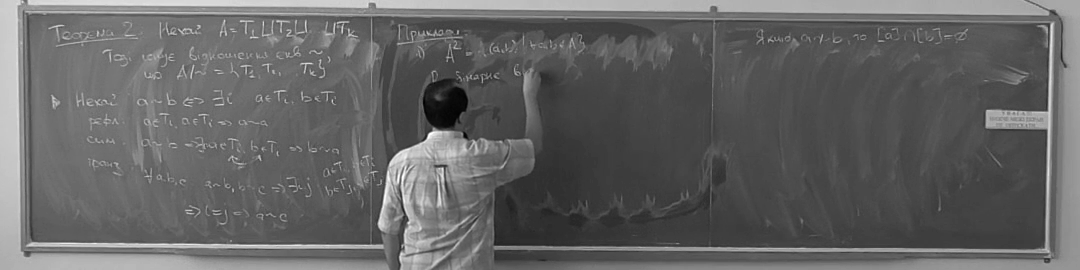
\includegraphics[width=\textwidth]{images/next_yakovlev}
        \caption{Поточний кадр
        \label{fig:yakovlev:bk_examples:b}
        }
    \end{subfigure}
\end{figure}
\begin{figure}[H]
    \centering
    \ContinuedFloat
    \begin{subfigure}[b]{0.55\textwidth}
        \centering
        
\includegraphics[width=\textwidth]{images/inv_diff}
        \caption{Інвертована різниця попереднього і поточного кадрів
        \label{fig:yakovlev:bk_examples:c}
        }
    \end{subfigure}

    \begin{subfigure}[b]{0.55\textwidth}
        \centering
        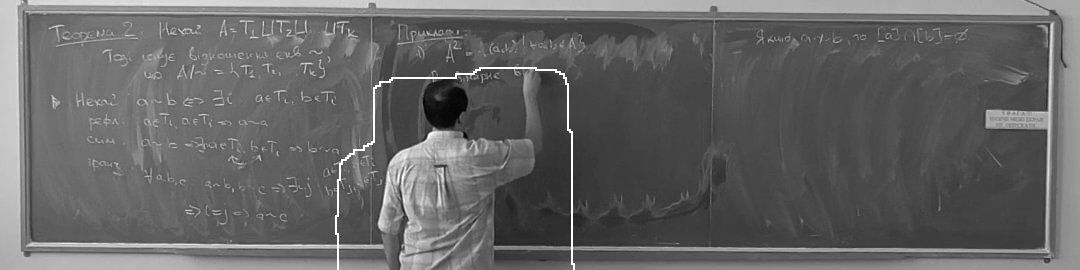
\includegraphics[width=\textwidth]{images/mask_yakovlev}
        \caption{Маска рухомих об'єктів
        \label{fig:yakovlev:bk_examples:d}
        }
    \end{subfigure}

    \caption{Процес створення маски з відео
    \label{fig:yakovlev:bk_examples}
    }
\end{figure}


Для того, щоб видалити всі рухомі об'єкти, які можуть перекривати дошку, ми
беремо кадри \(F^{i}\) та \(F^{i + s}\)  ( рис. \ref{fig:yakovlev:bk_examples}, 
\subref{fig:yakovlev:bk_examples:a},
\subref{fig:yakovlev:bk_examples:b}) та для
кожної пари кольорів пікселів \(p\) з однаковими координатами знаходимо
модуль \(D_{p}^{i} = \left| F_{p}^{i} - F_{p}^{i + s} \right|\) різниці
інтенсивностей (Рис. 2 (в)). Зображення \(D^{i}\) подаємо на вхід
алгоритму Бойкова-Колмогорова.

Треба знайти маску \(B^{i}:P \rightarrow \left\{ 0,1 \right\}\) рухомих
об'єктів для кадрів \(F^{i}\) і \(F^{i + s}\). 
Введемо функції.